%!TEX root = ../thesis.tex
%%%%%%%%%%%%%%%%%%%%%%%%%%%%%%%%%%%%%%%%%%%%%%%%%%%%%%%%%%%%%%%%%%%%%%%
%
% System Architecture
%
%%%%%%%%%%%%%%%%%%%%%%%%%%%%%%%%%%%%%%%%%%%%%%%%%%%%%%%%%%%%%%%%%%%%%%%
\chapter{System Architecture}%
\chaptermark{System Architecture}%
\label{chapter:system_architecture}

\section{Application Architecture}

\begin{figure}[!hb]
\centering
\caption[Application Architecture]{Application Architecture}%
\label{fig:application_architecture}
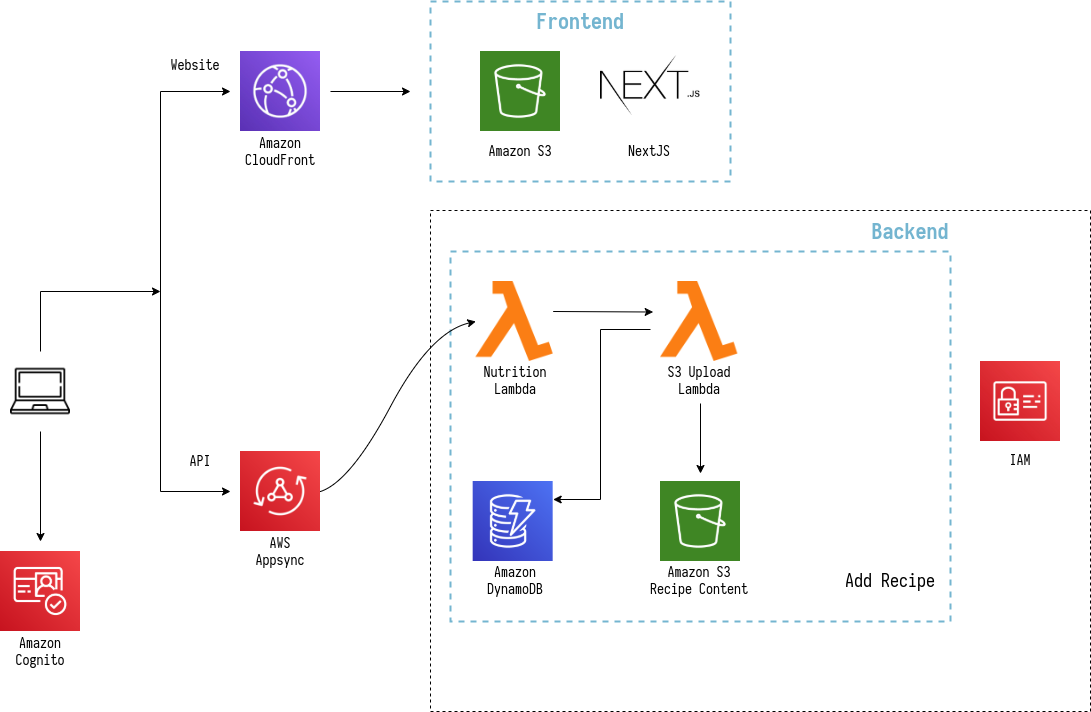
\includegraphics[width=\linewidth,height=\textheight,keepaspectratio]{img/application_architecture}
\end{figure}

\clearpage

\section{ER Diagram}

\begin{figure}[!hb]
\centering
\caption[ER Diagram]{ER Diagram}%
\label{fig:erd}
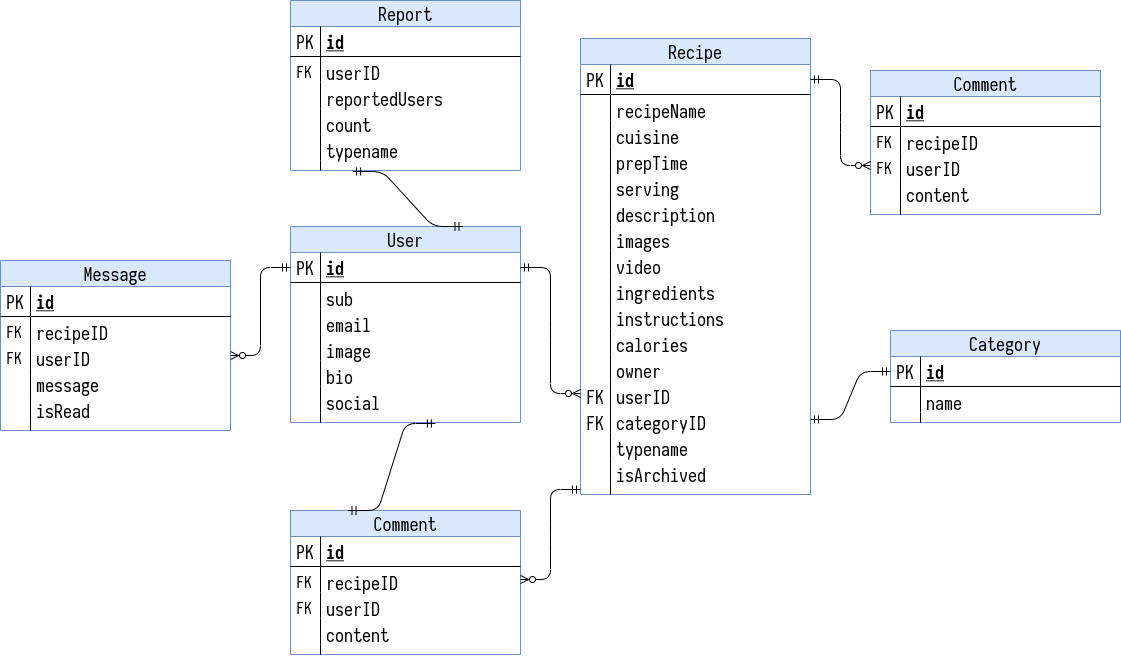
\includegraphics[width=\linewidth,height=\textheight,keepaspectratio]{img/erd}
\end{figure}

\clearpage

\section{Use Case Diagram}

\begin{figure}[!hb]
\centering
\caption[Use Case Diagram]{Use Case Diagram}%
\label{fig:use_case_diagram}
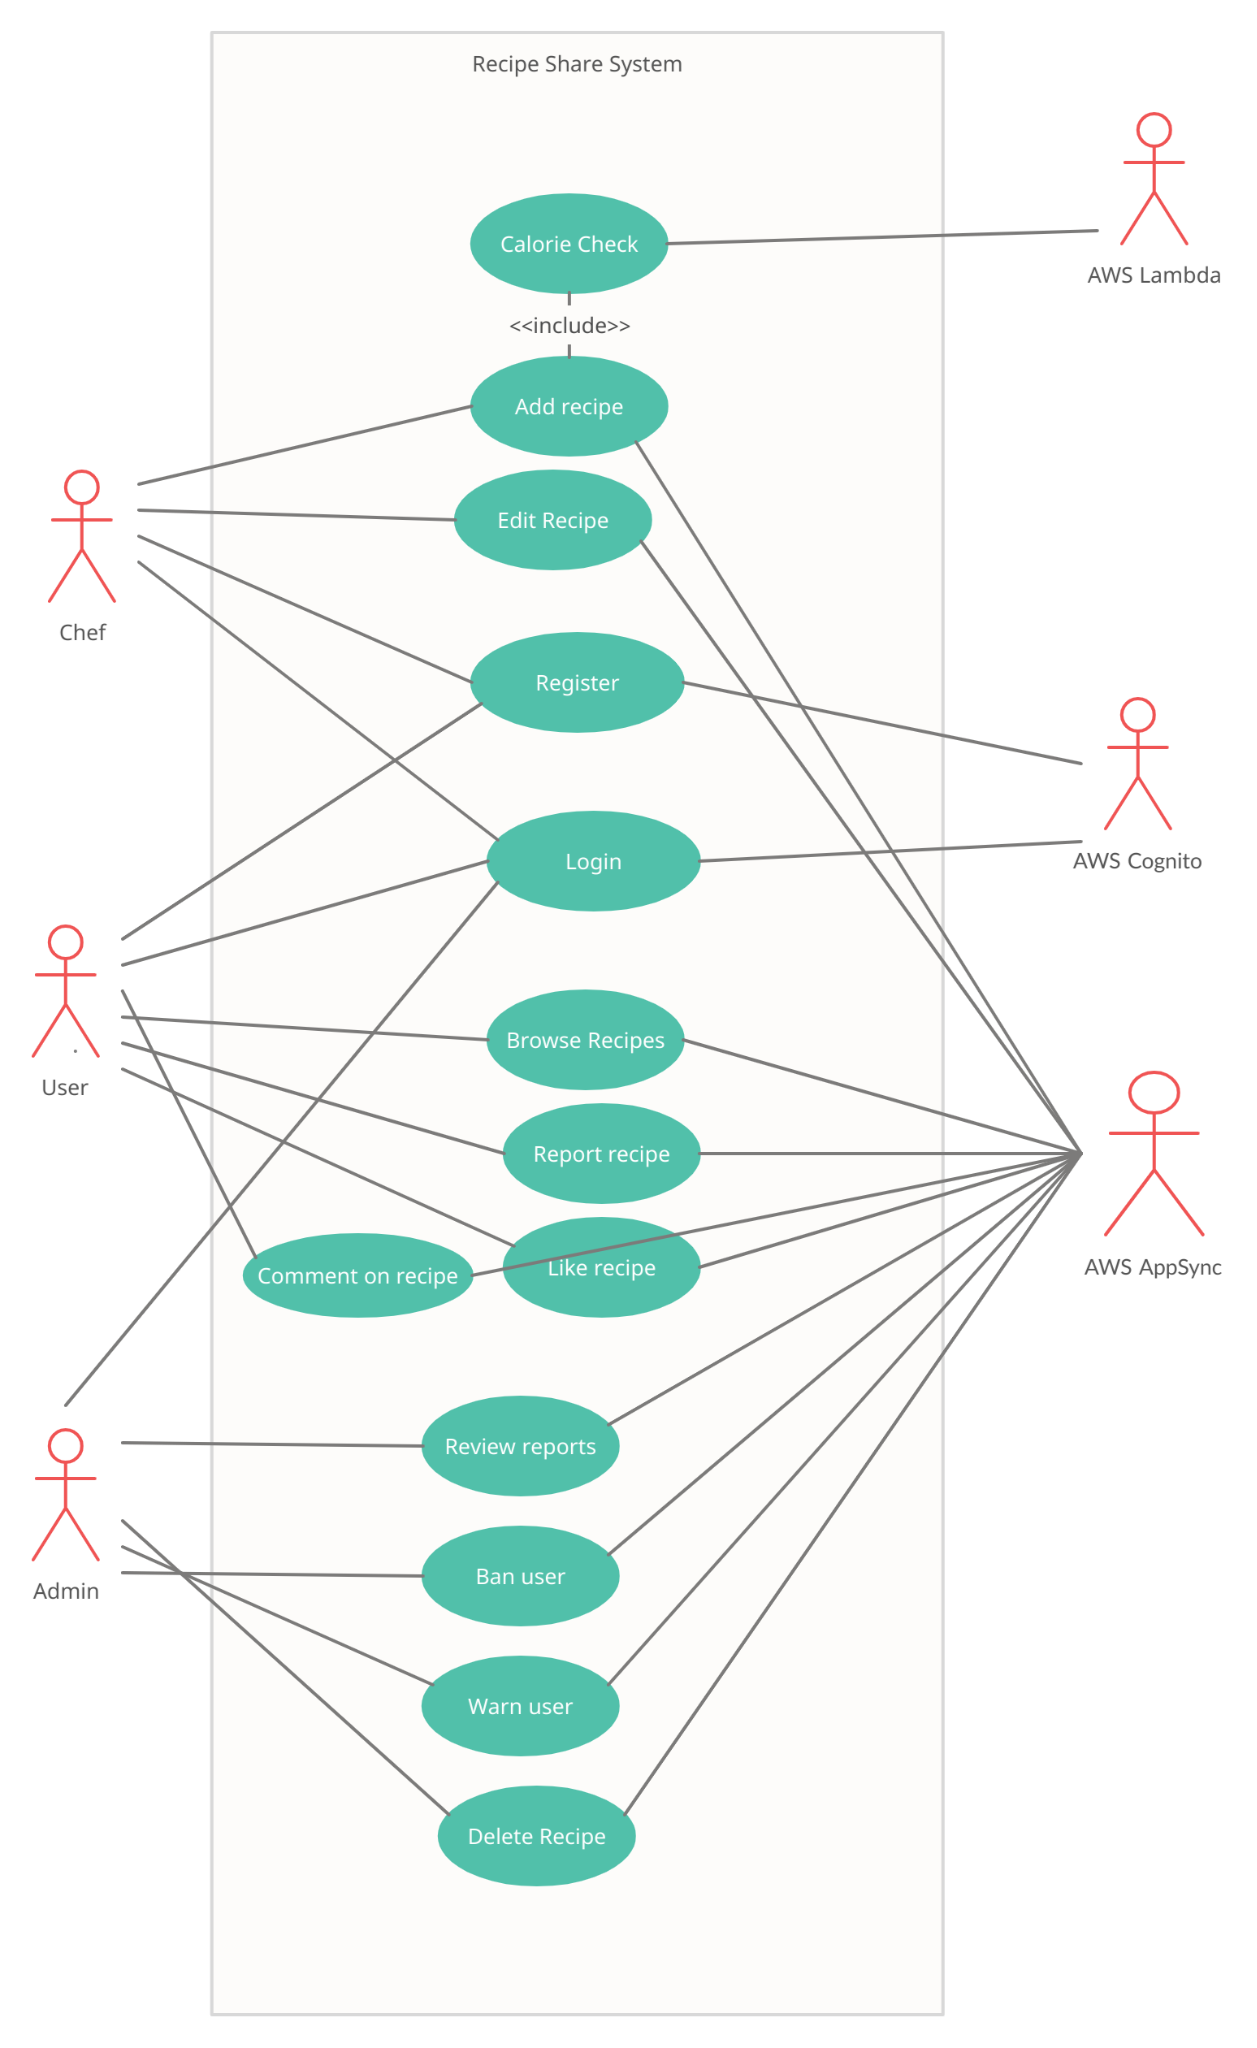
\includegraphics[width=\linewidth,height=20cm,keepaspectratio]{img/use_case_diagram}
\end{figure}

\clearpage

\section{Activity Diagram}

\begin{figure}[!hb]
\centering
\caption[Activity Diagram]{Activity Diagram}%
\label{fig:activity_diagram}
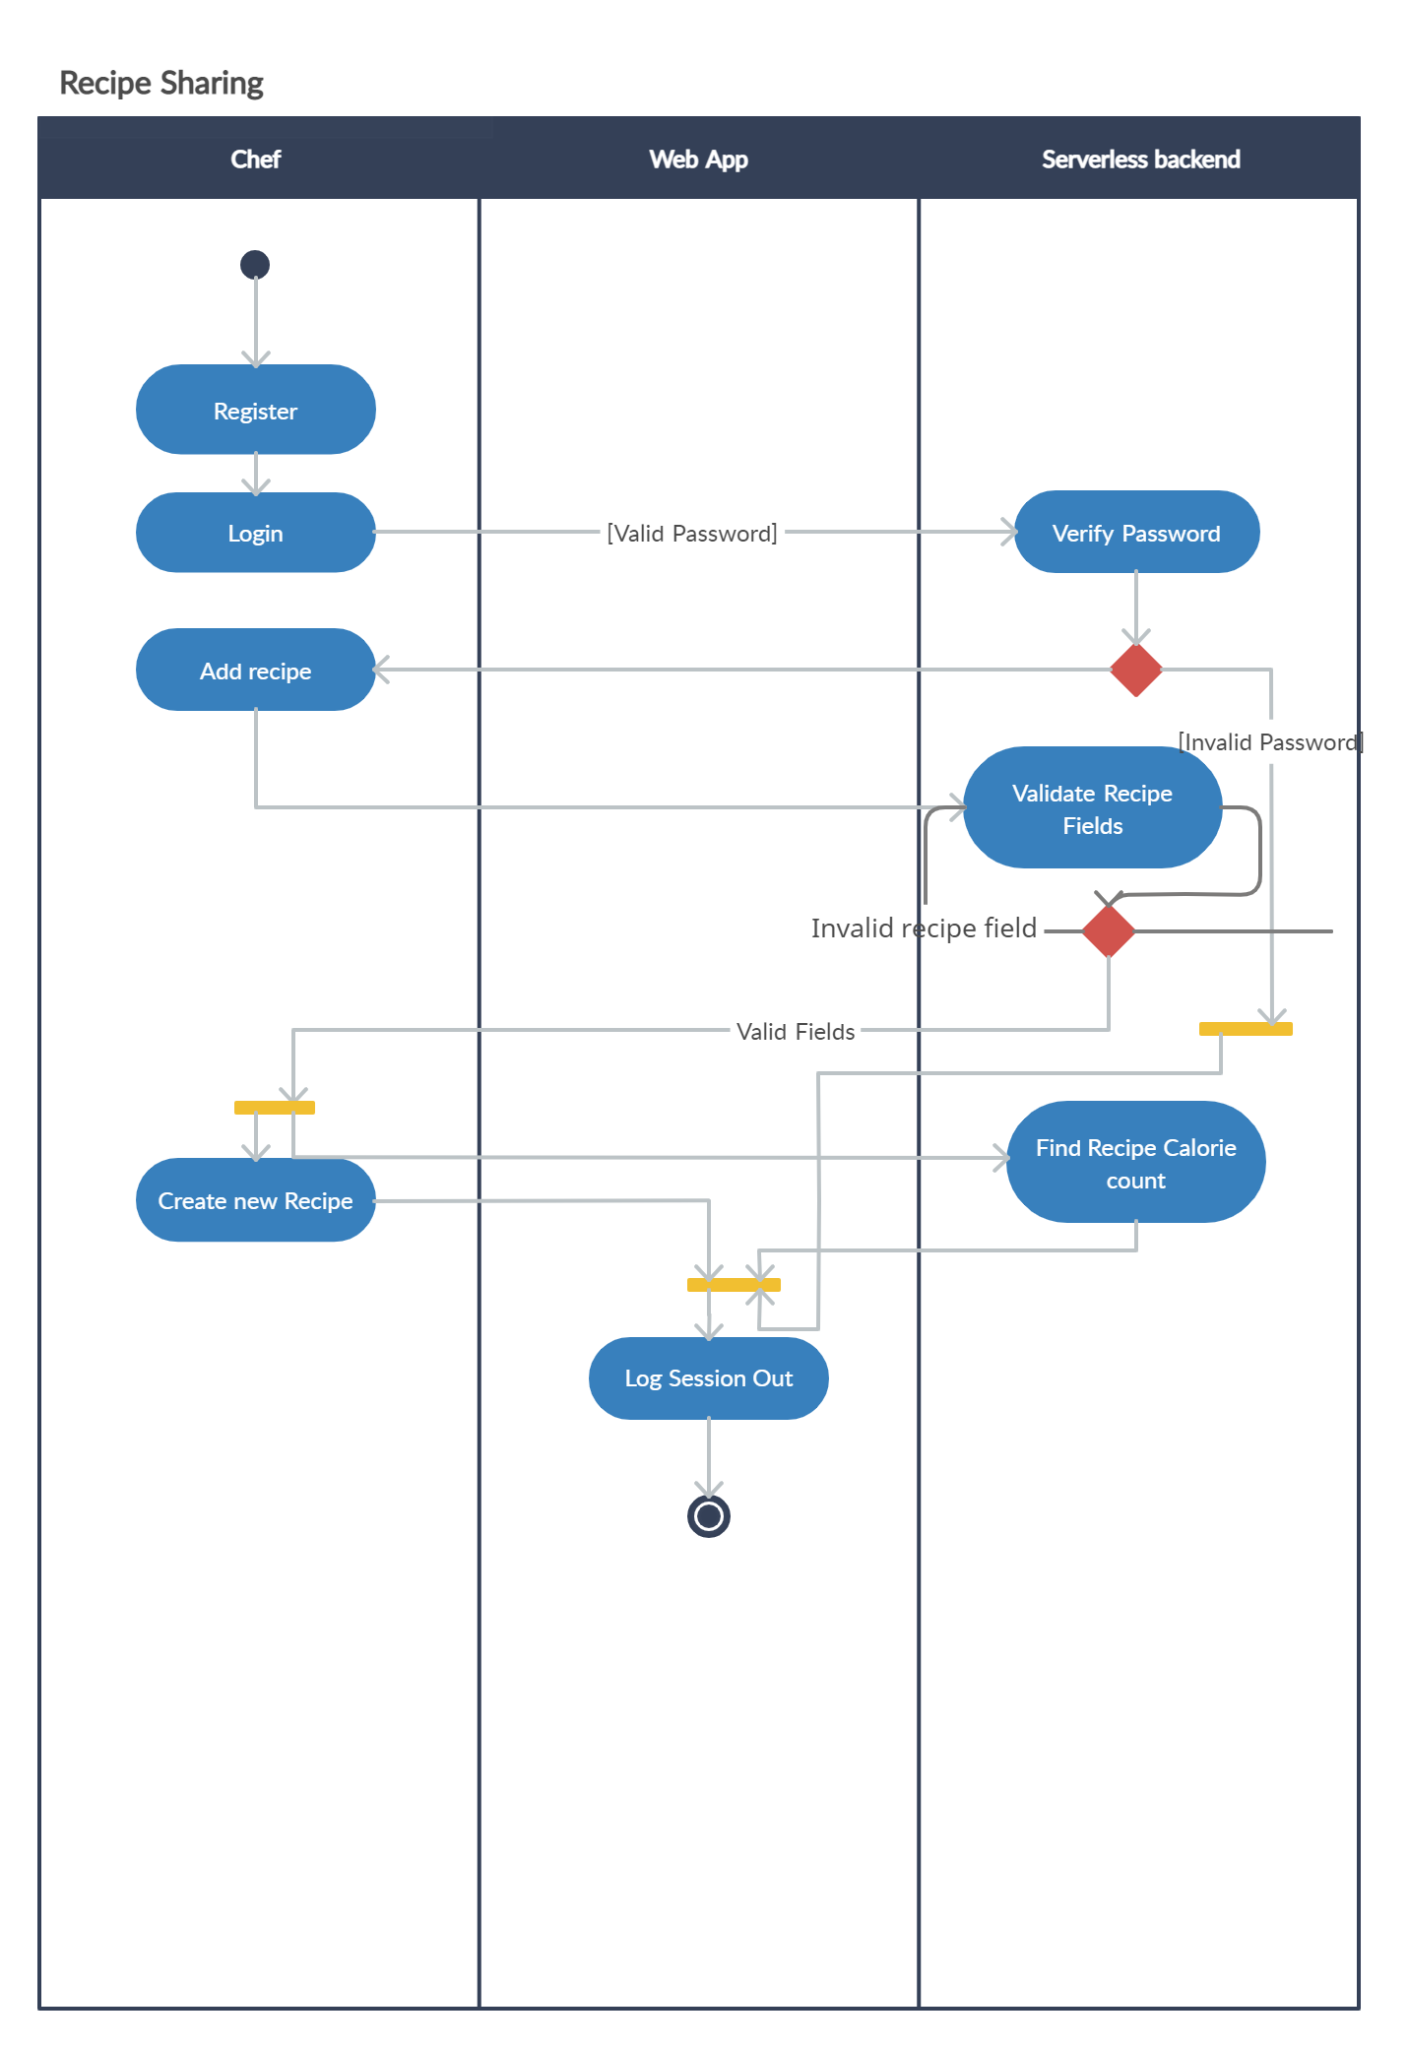
\includegraphics[width=\linewidth,height=20cm,keepaspectratio]{img/activity_diagram}
\end{figure}

\section{User Interface Design}

Most of our design needs custom CSS to achieve the desired look. Depending solely on a UI library would rid the website of its uniqueness, making it lacklustre. 

\begin{figure}[!hb]
\centering
\caption[Header Section]{Header Section}%
\label{fig:header_section}
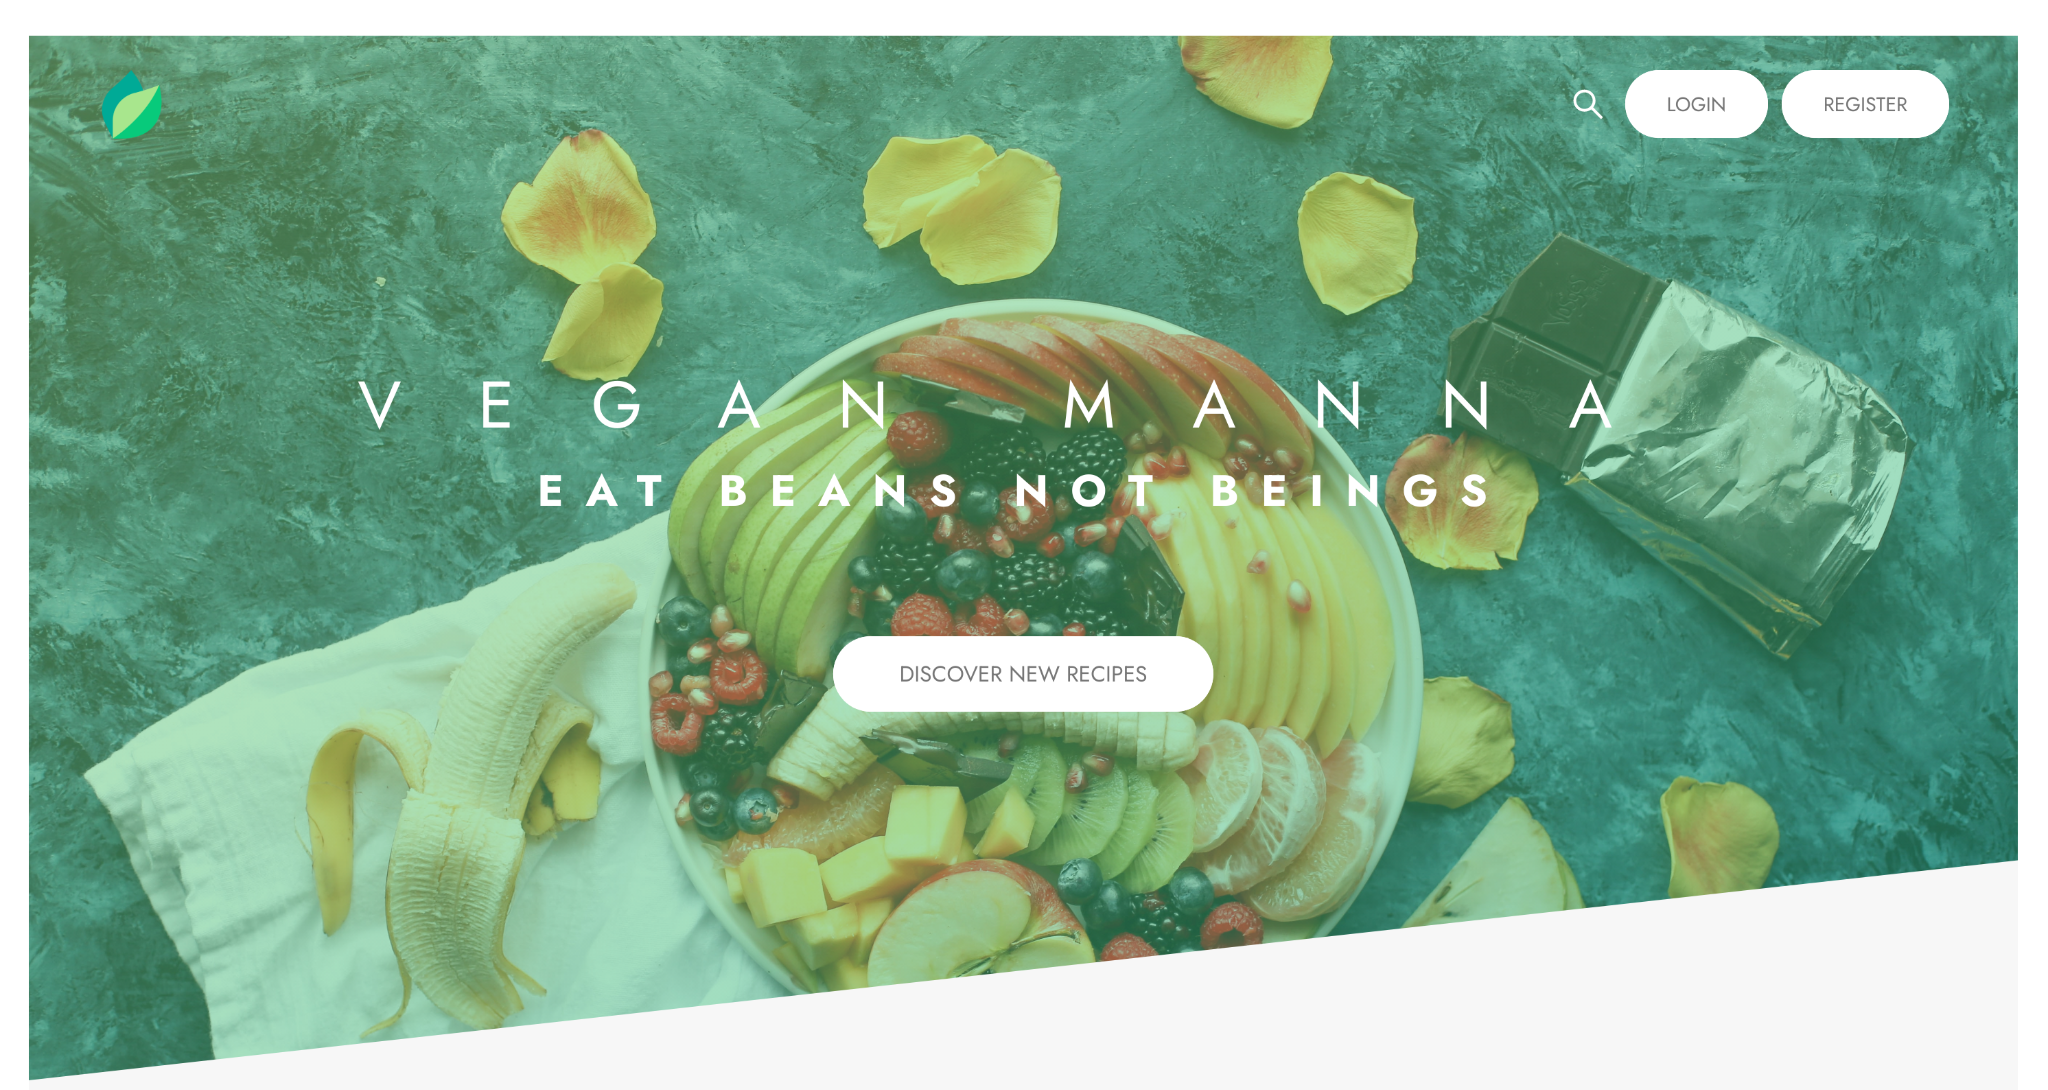
\includegraphics[width=\linewidth,height=20cm,keepaspectratio]{img/header_section}
\end{figure}

The above effect of the header section is achieved using the clip-path of CSS, into a polygon.

\begin{figure}[!hb]
\centering
\caption[About Section]{About Section}%
\label{fig:about_section}
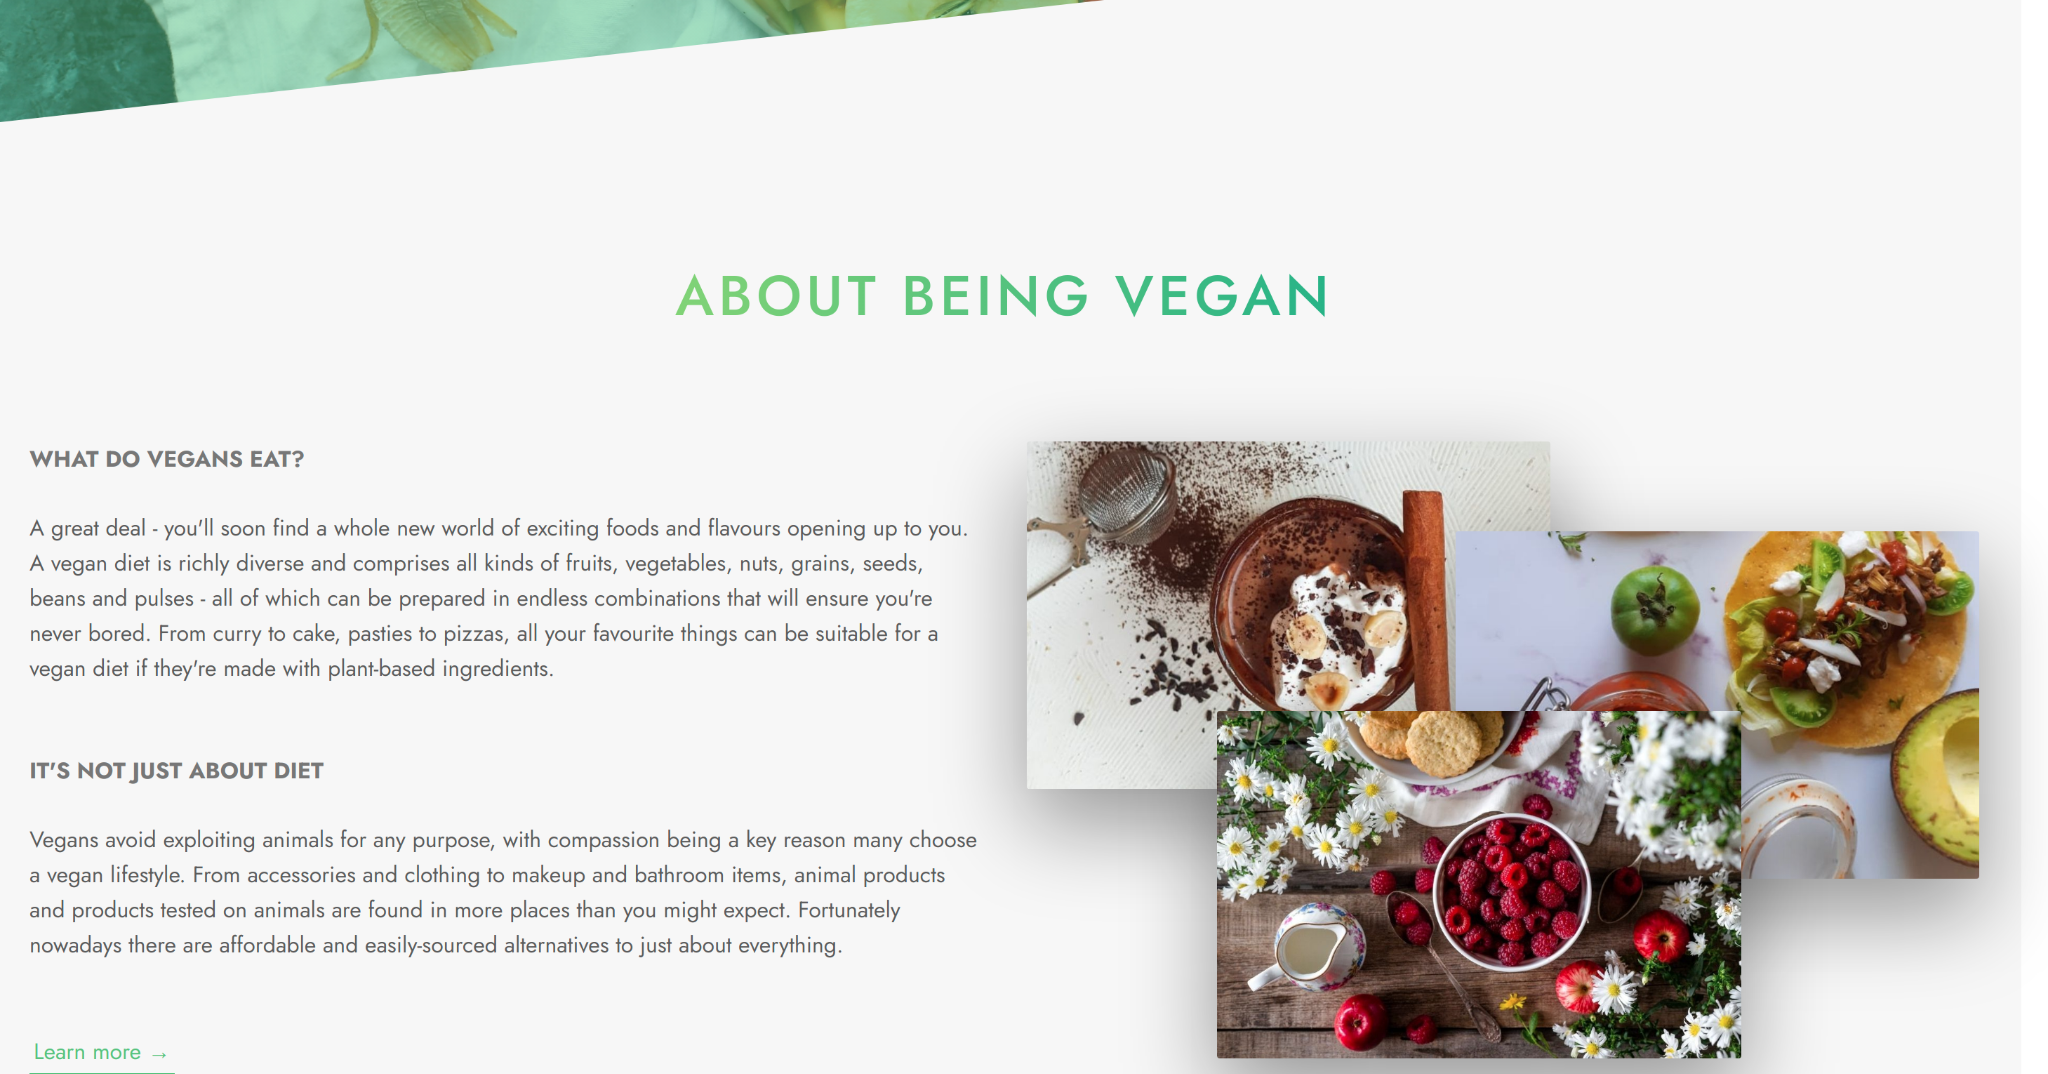
\includegraphics[width=\linewidth,height=20cm,keepaspectratio]{img/about_section}
\end{figure}

\clearpage

\begin{figure}[!hb]
\centering
\caption[Image Collage]{Image Collage}%
\label{fig:image_collage}
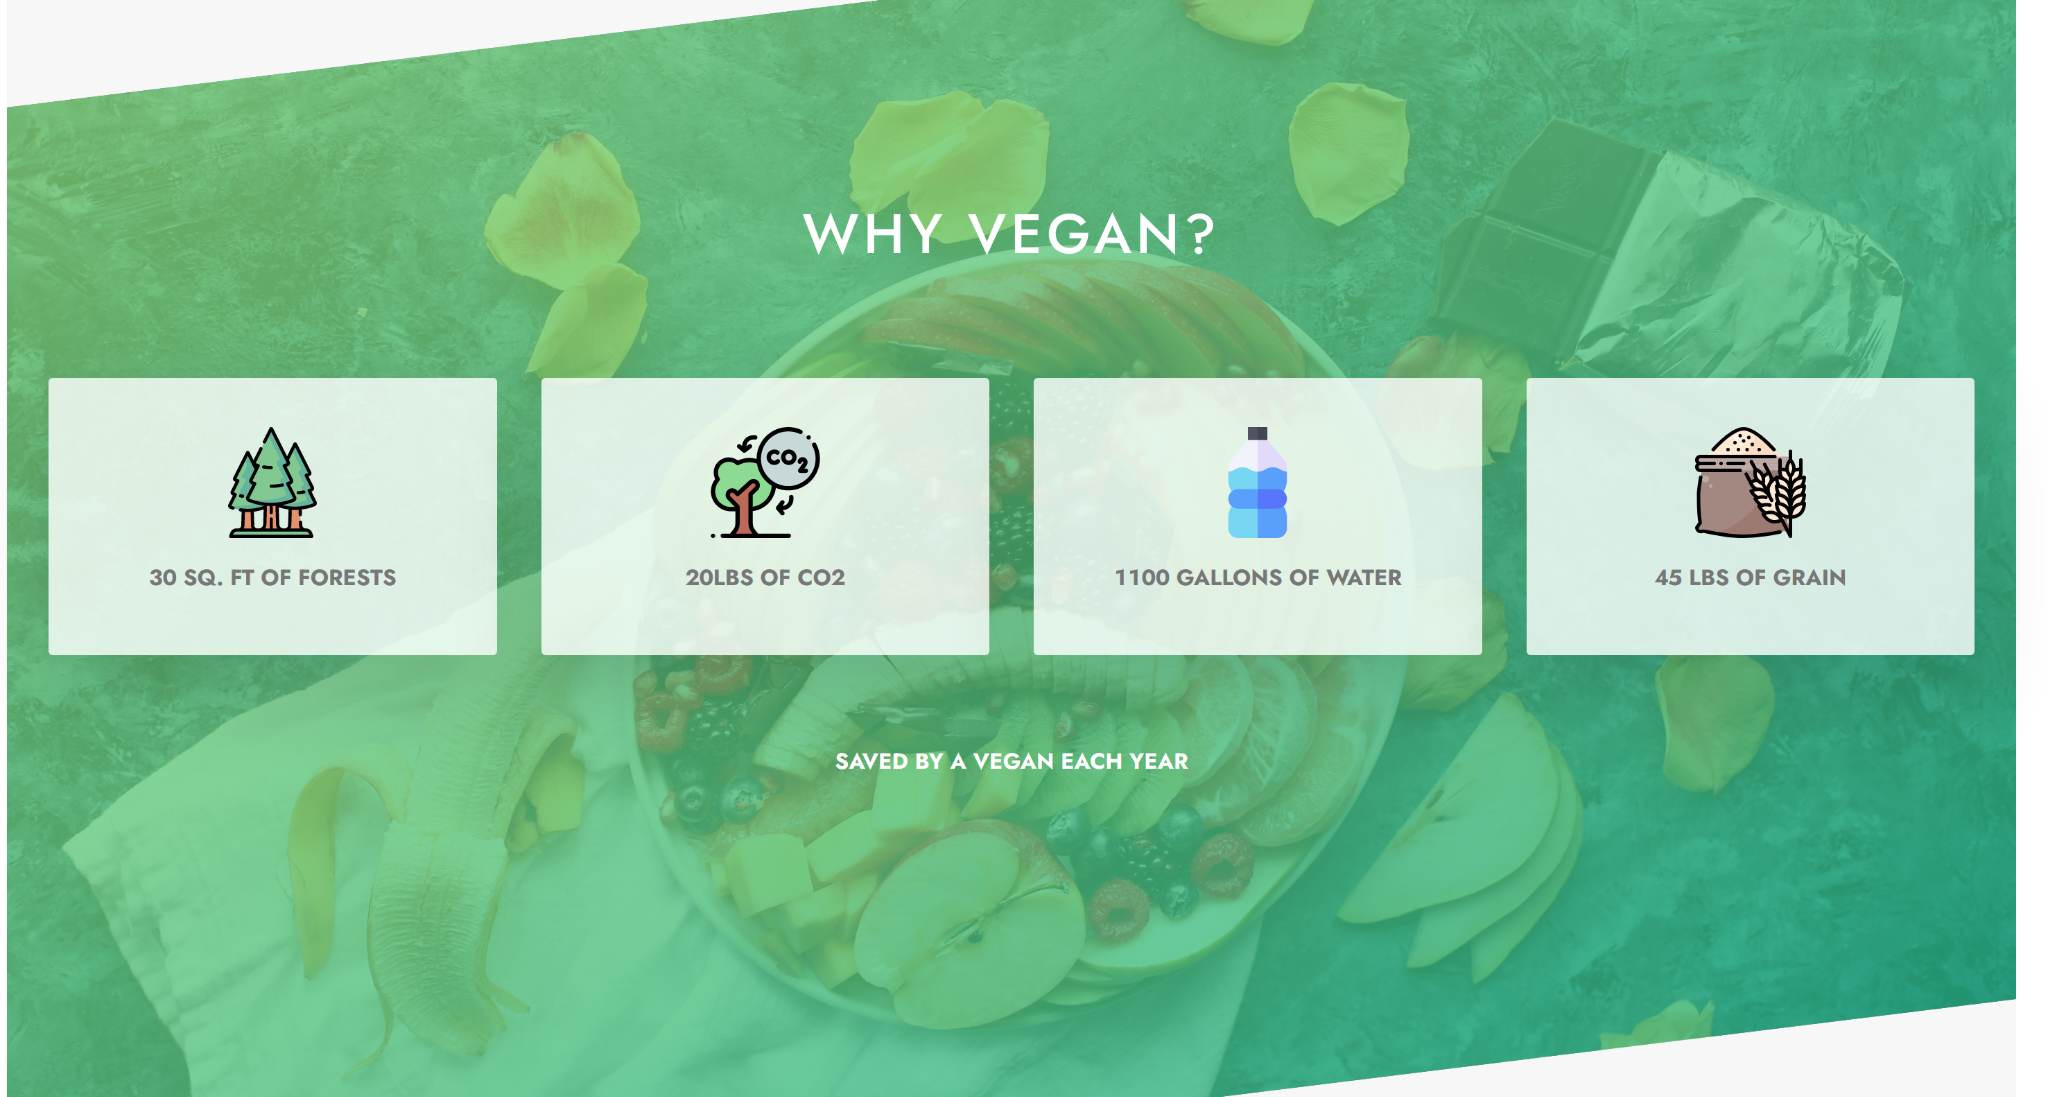
\includegraphics[width=\linewidth,height=20cm,keepaspectratio]{img/image_collage}
\end{figure}

The animations for the image collage as well as the call to action cards are implemented using only css transitions, on the hover state.

\begin{figure}[!hb]
\centering
\caption[Recipe Card]{Recipe Card}%
\label{fig:recipe_card}
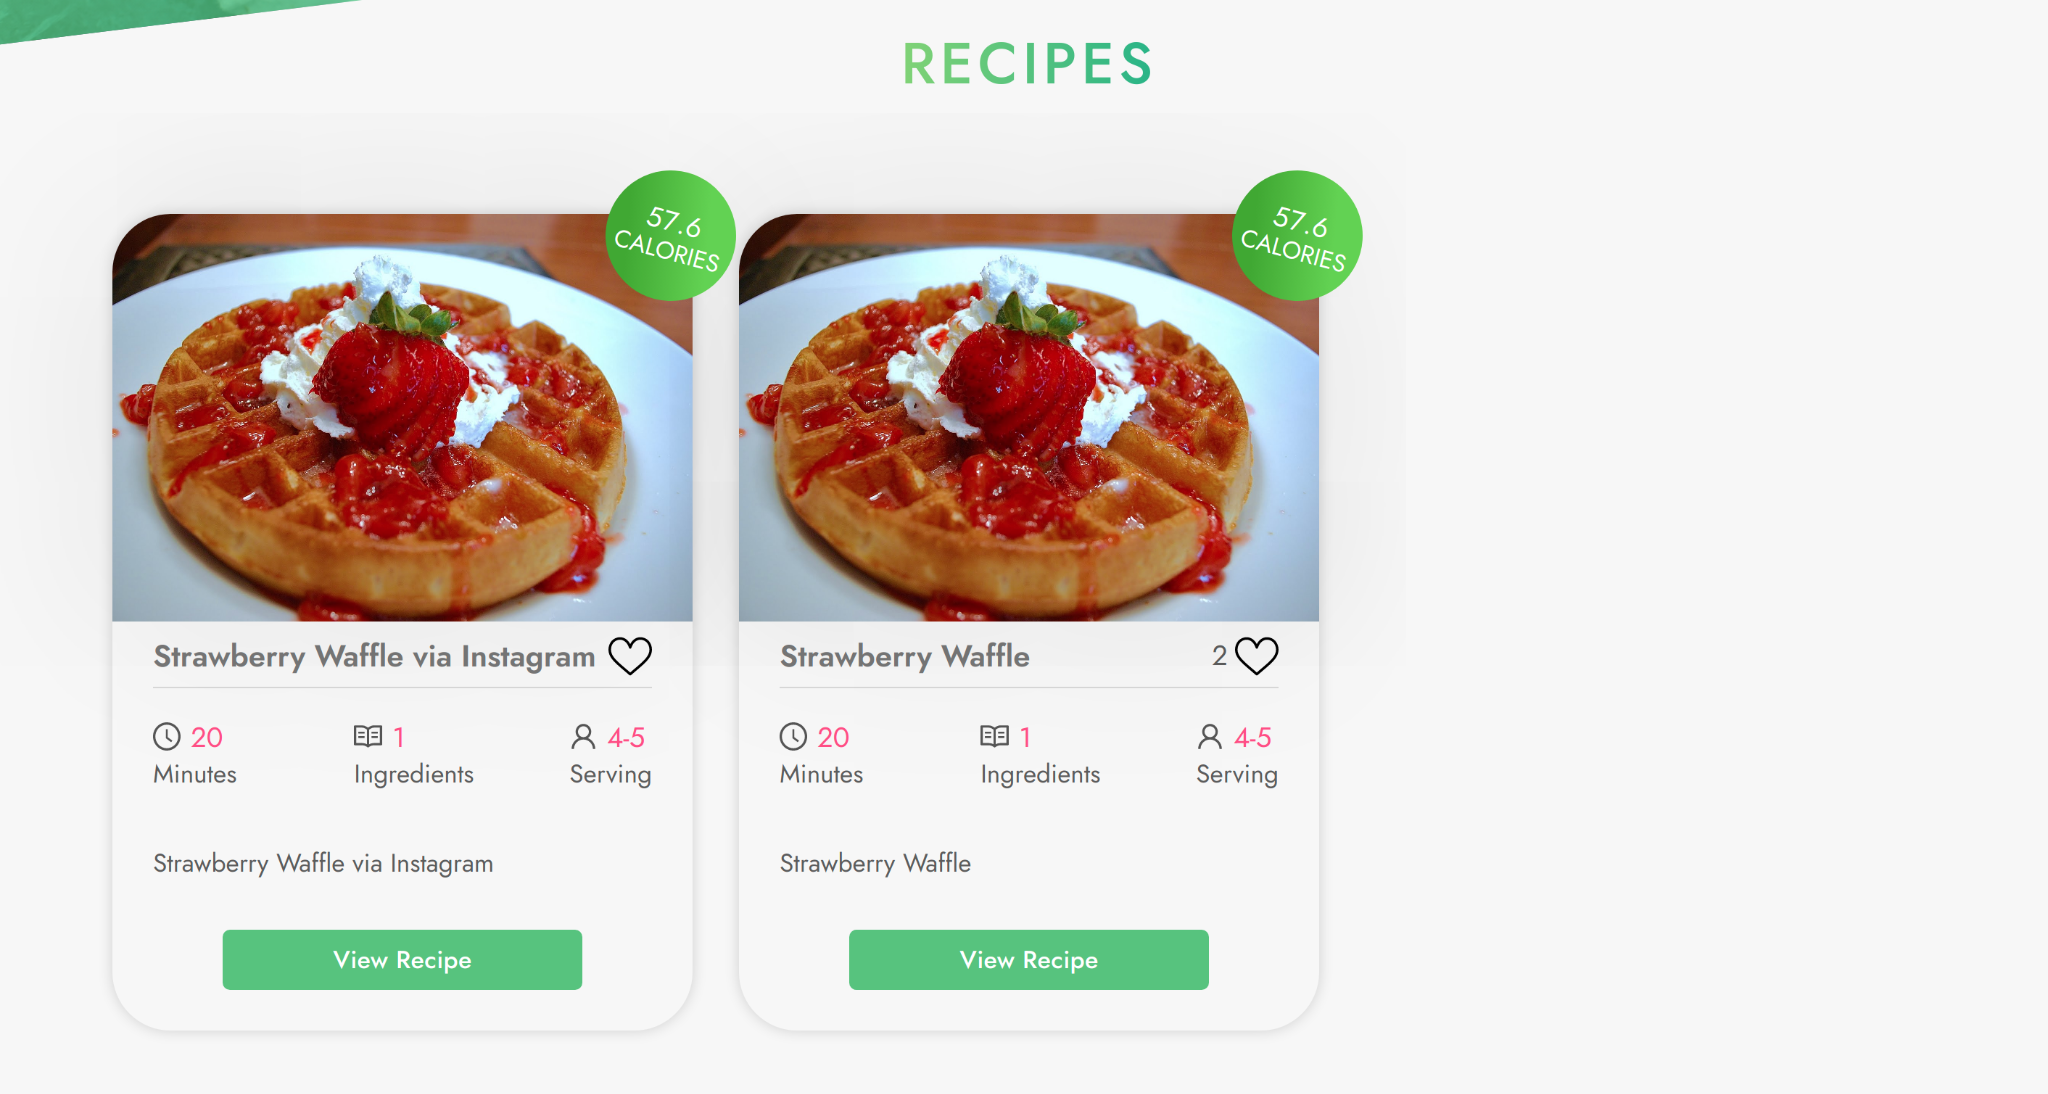
\includegraphics[width=\linewidth,height=20cm,keepaspectratio]{img/recipe_card}
\end{figure}

The cards are built using only CSS, using flexbox.

\clearpage

\begin{figure}[!hb]
\centering
\caption[Footer Section]{Footer Section}%
\label{fig:footer_section}
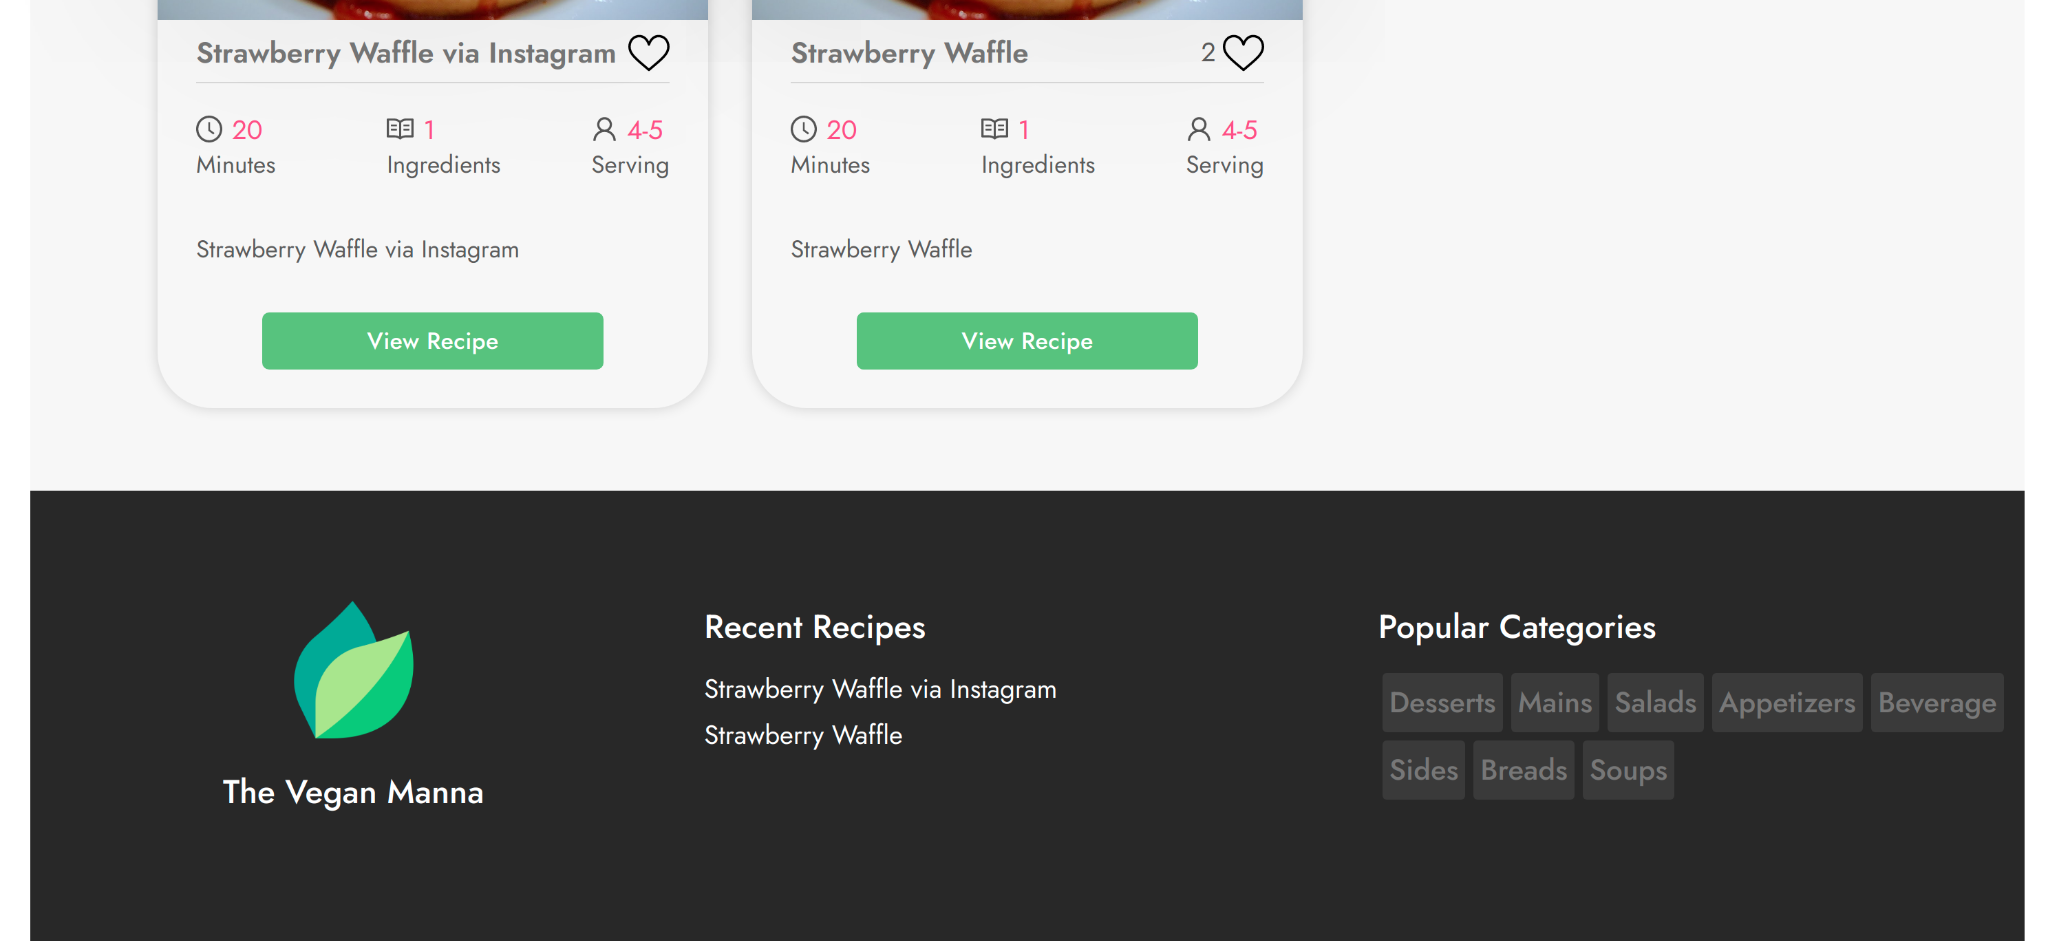
\includegraphics[width=\linewidth,height=20cm,keepaspectratio]{img/footer_section}
\end{figure}

We use Flexbox for laying out the internal structure of UI components like the footer. 

\begin{figure}[!hb]
\centering
\caption[Login UI]{Login UI}%
\label{fig:login_ui}
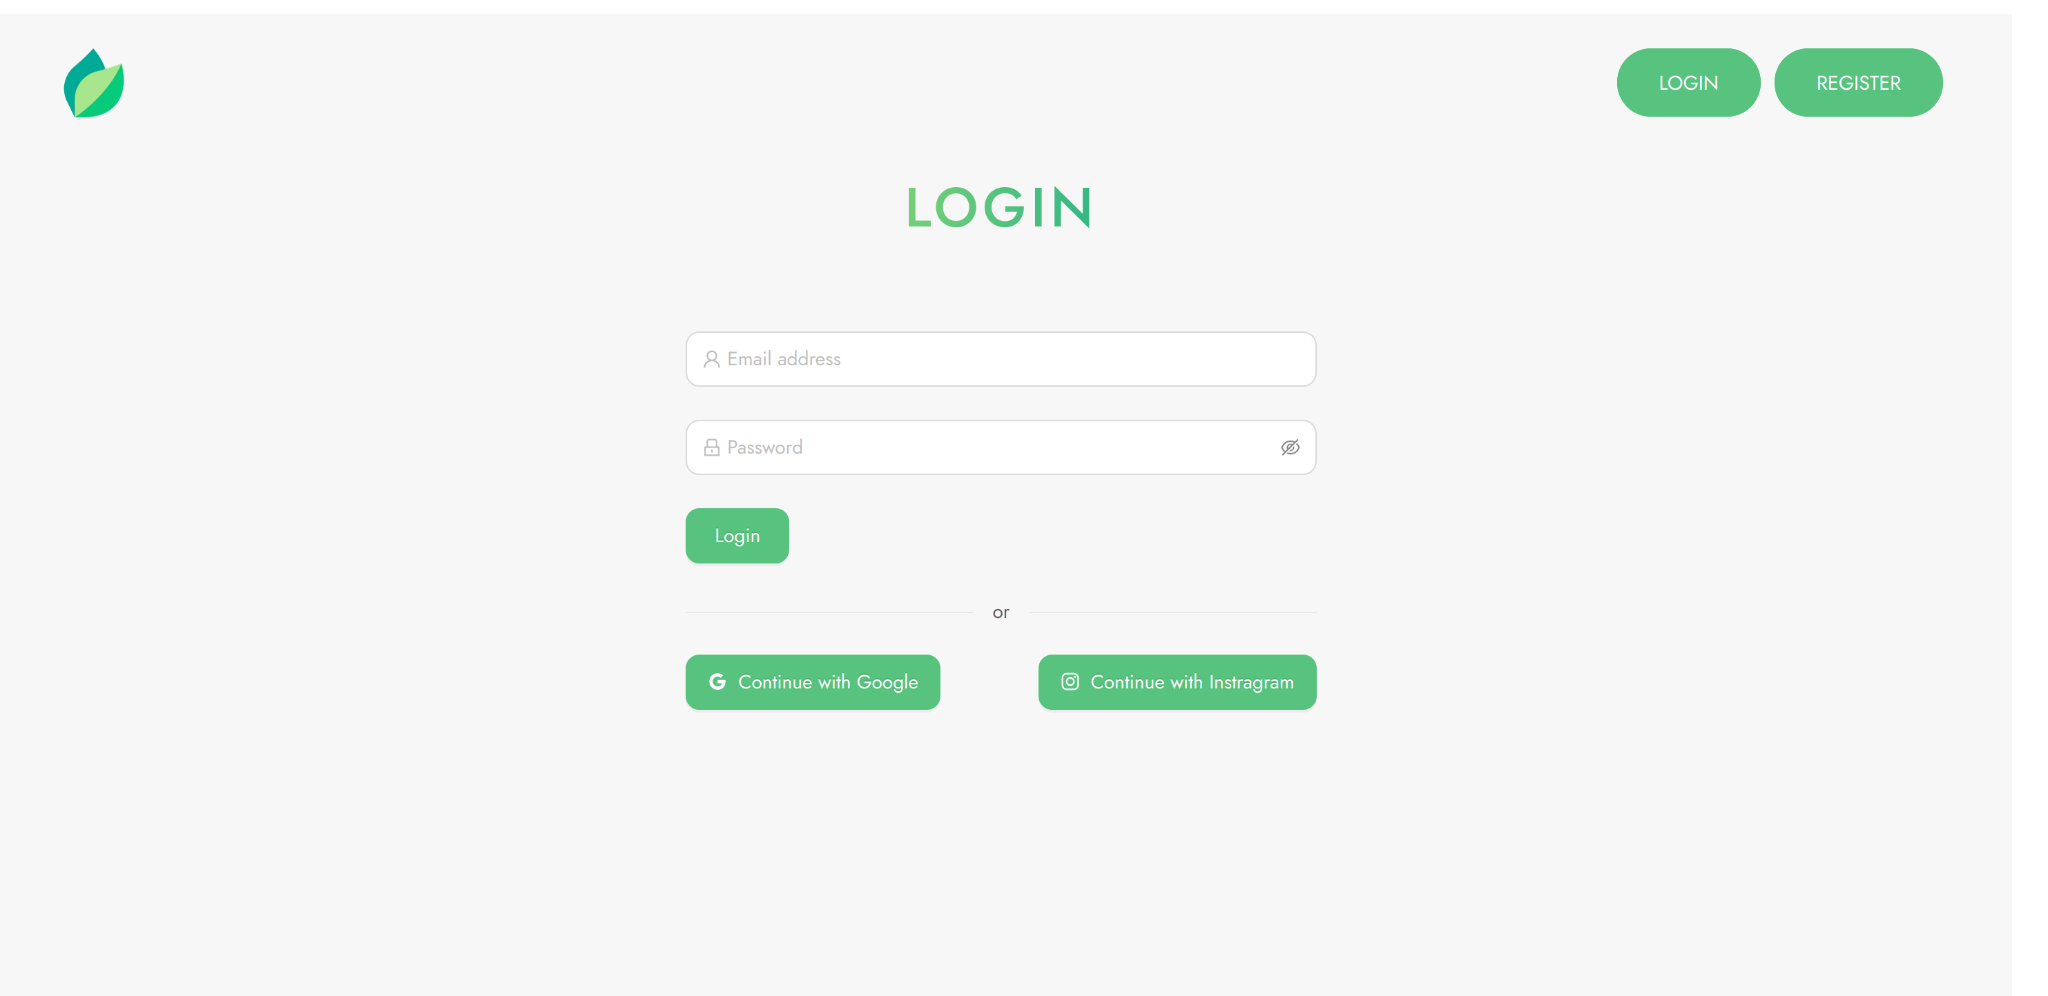
\includegraphics[width=\linewidth,height=20cm,keepaspectratio]{img/login_ui}
\end{figure}

We use Ant design for the login and register fields. 

\clearpage

\begin{figure}[!hb]
\centering
\caption[Register UI]{Register UI}%
\label{fig:register_ui}
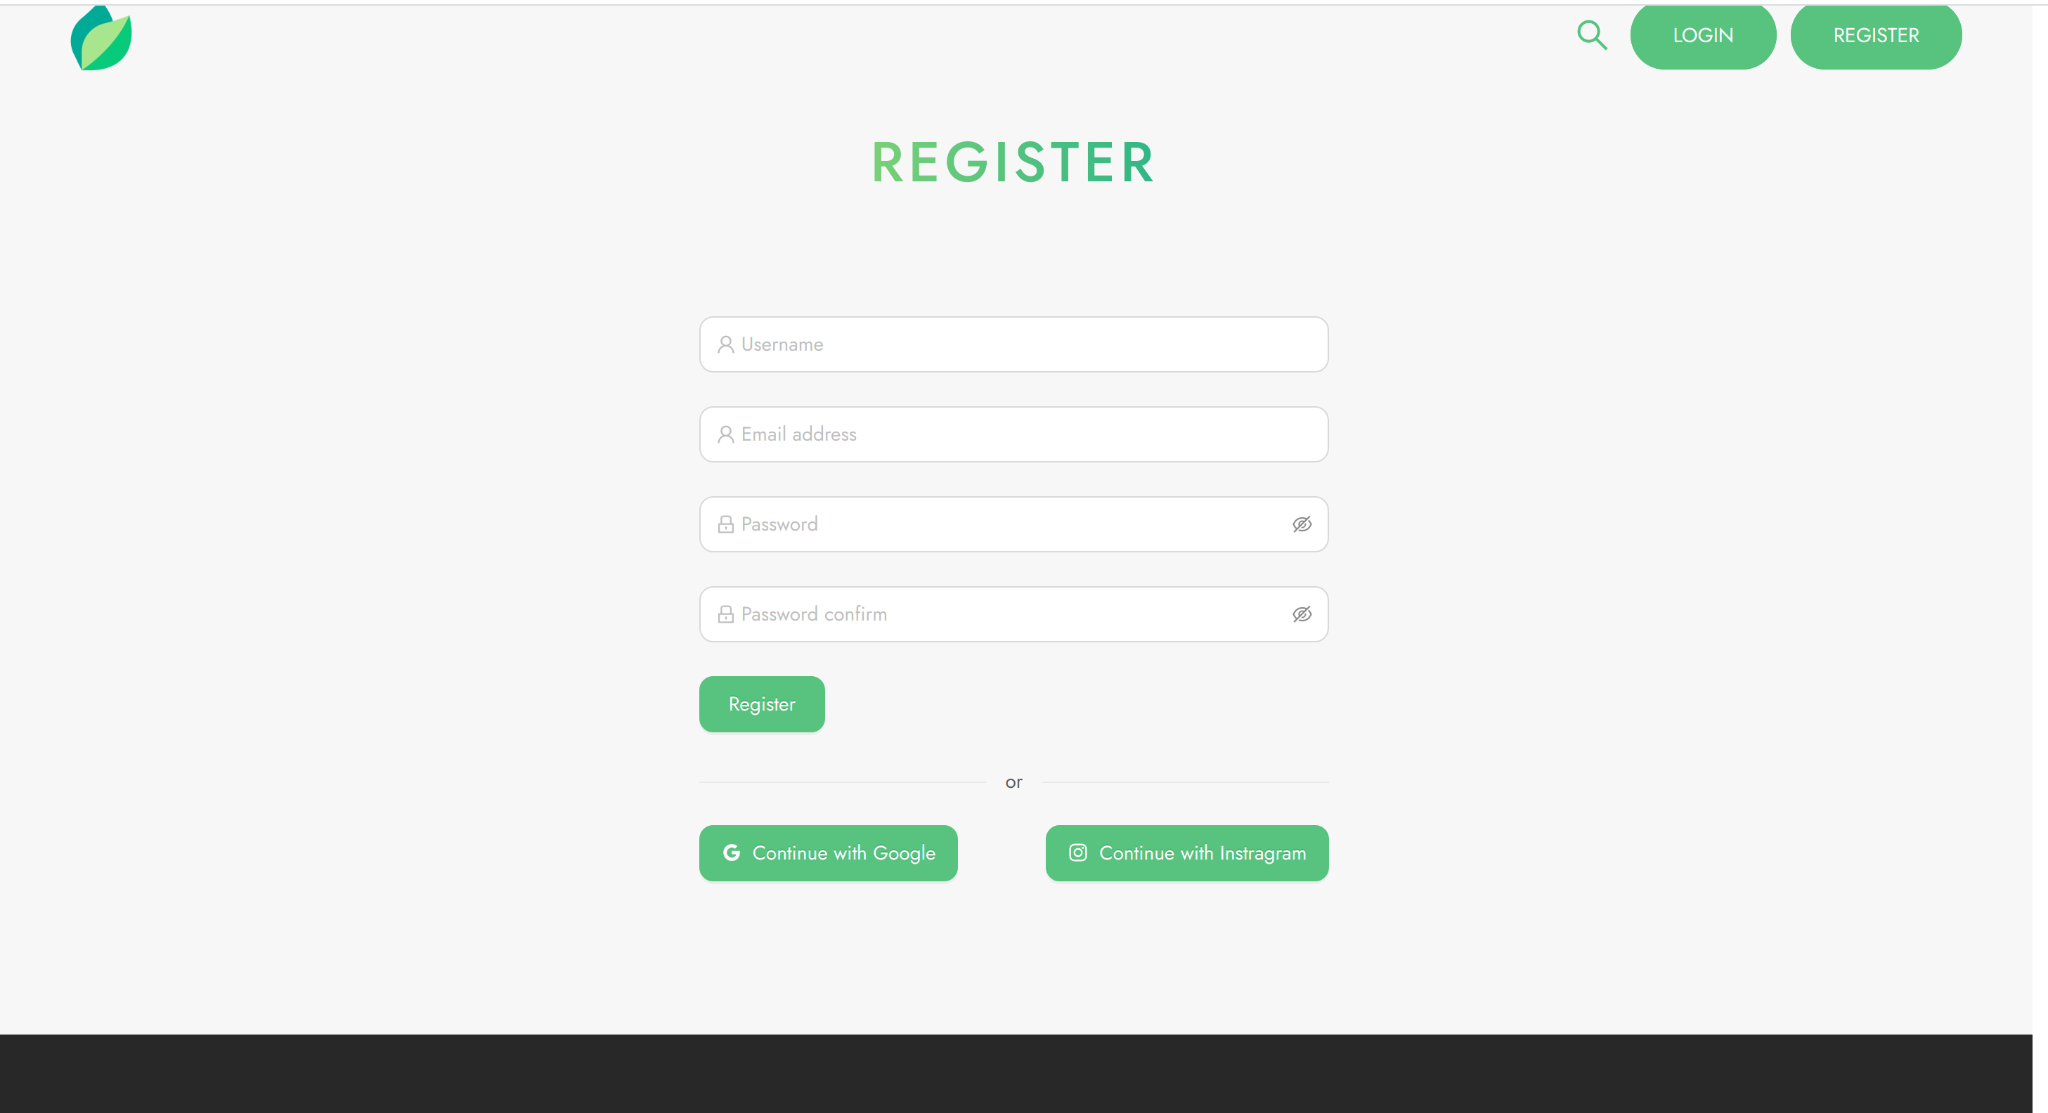
\includegraphics[width=\linewidth,height=20cm,keepaspectratio]{img/register_ui}
\end{figure}

\begin{figure}[!hb]
\centering
\caption[Search bar]{Search bar}%
\label{fig:search_bar}

\includegraphics[width=\linewidth,height=20cm,keepaspectratio]{img/search_bar}
\end{figure}

We also have a search bar implemented, which shows up only upon clicking 

\begin{figure}[!hb]
\centering
\caption[Recipe Detail]{Recipe Detail}%
\label{fig:recipe_detail}
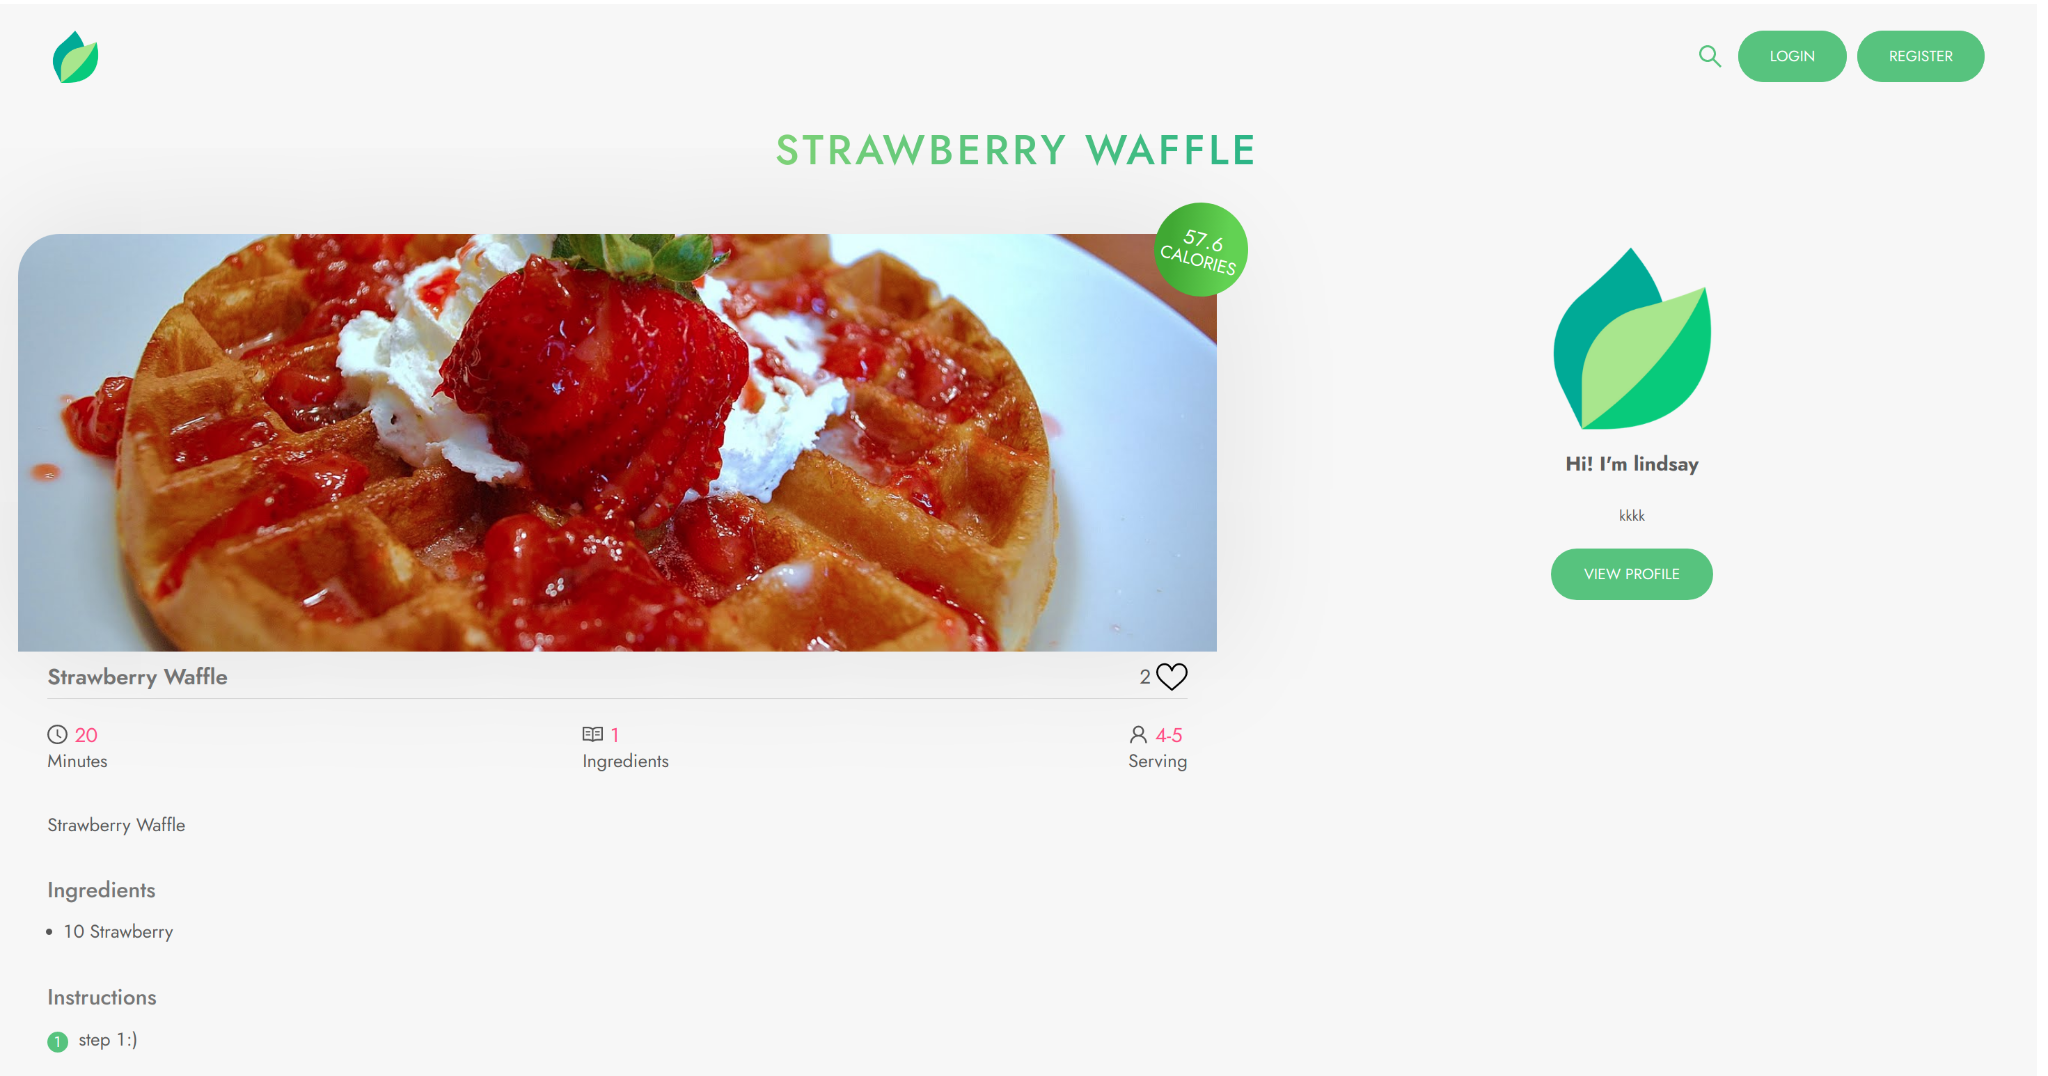
\includegraphics[width=\linewidth,height=20cm,keepaspectratio]{img/recipe_detail}
\end{figure}

The recipe details page is similar to our card design, with a link to the respective user profile added. 

\begin{figure}[!hb]
\centering
\caption[Search UI]{Search UI}%
\label{fig:search_ui}
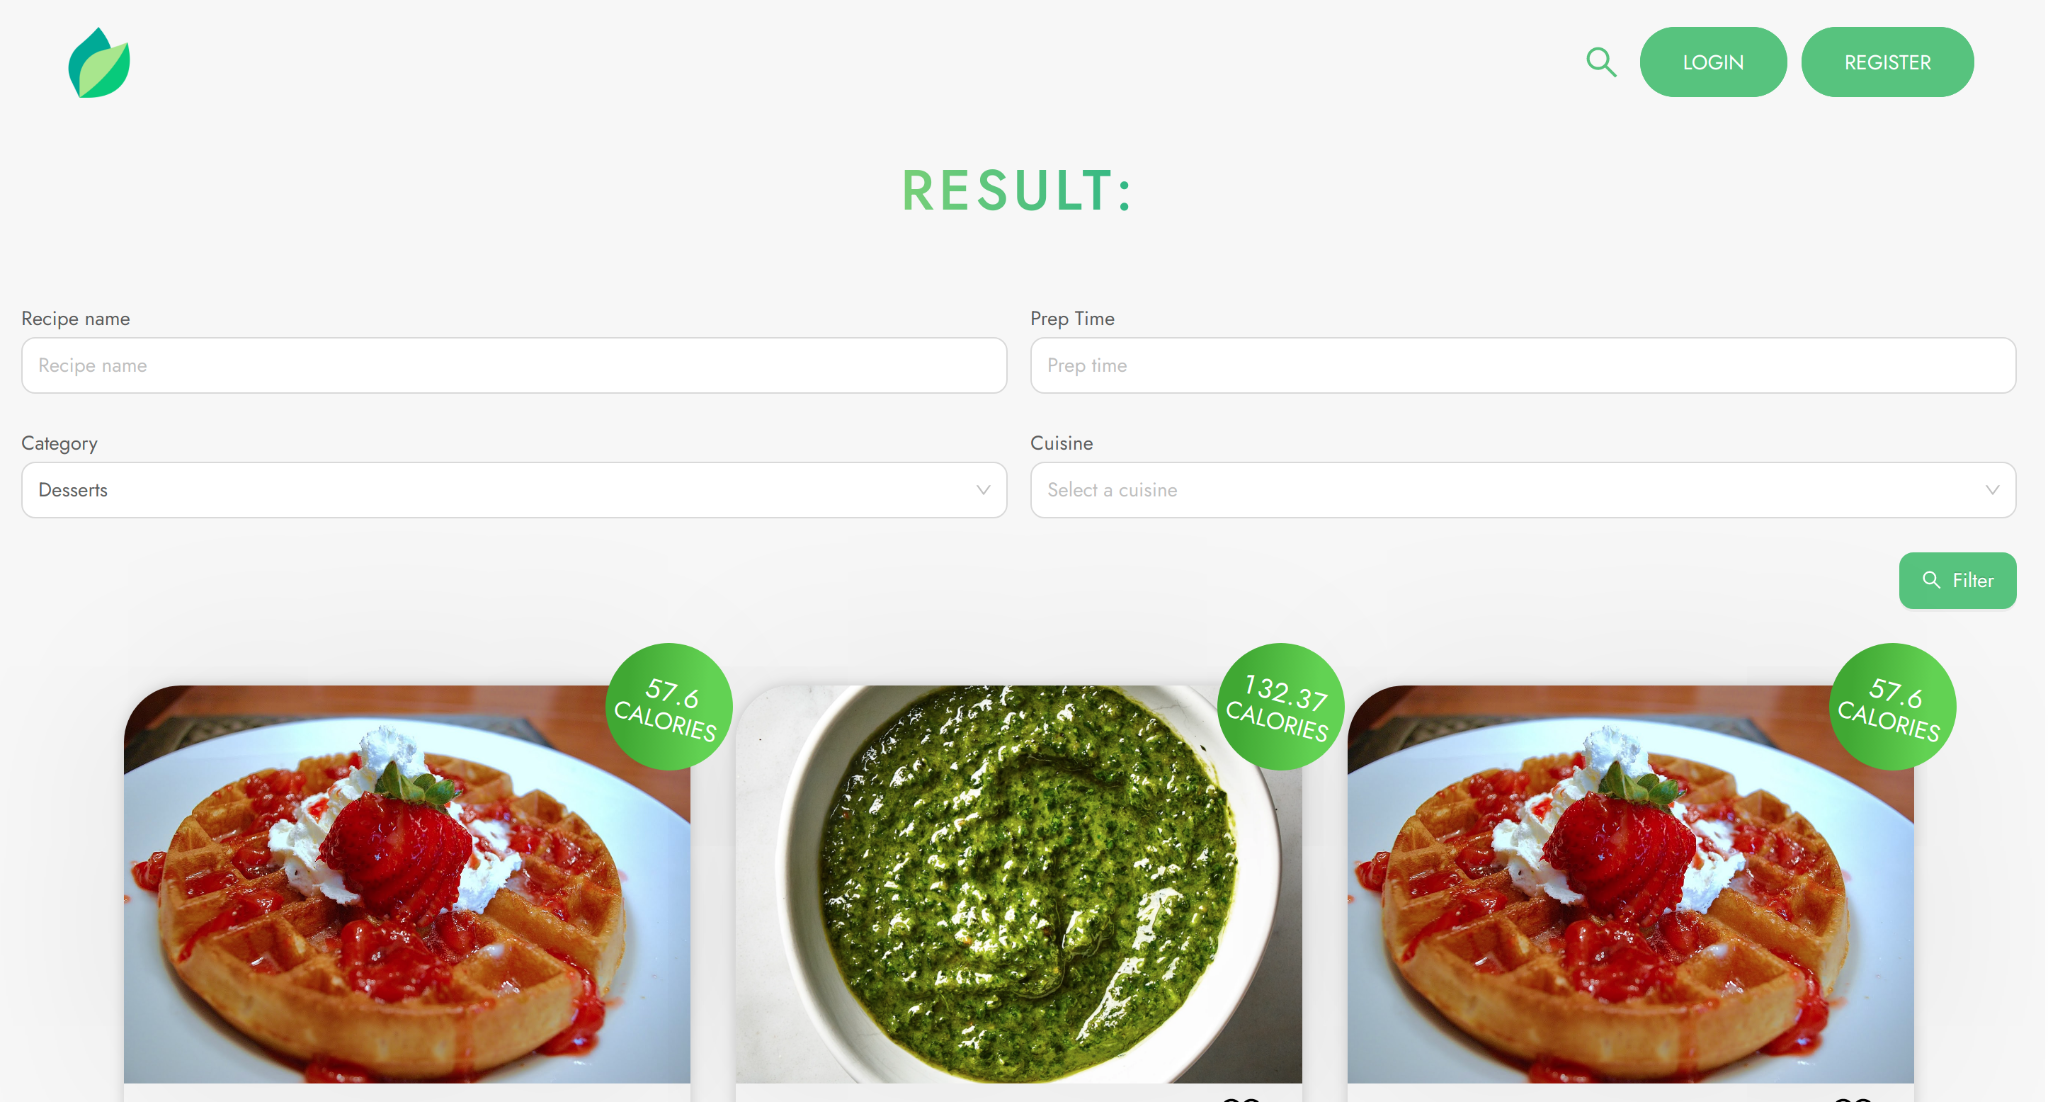
\includegraphics[width=\linewidth,height=20cm,keepaspectratio]{img/search_ui}
\end{figure}

We also have a page to filter out search results based on recipe name keywords, categories, preparation-time and cuisine. 



